\section{Background and Motivation}

\subsection{The Diversity of GPU-Centric Workloads}
% \xiangyu{Workloads in CPU clusters}

Modern GPU-centric systems, ranging from single-node dense servers to disaggregated clusters, host heterogeneous workloads with fundamentally conflicting resource requirements. Generative AI inference pipelines are increasingly complex: Prefill-Decode disaggregation separates compute-intensive prompt processing from bandwidth-bound token generation across networked nodes~\cite{zhong2024distserve,patel2024splitwise}; KV-cache offloading alternates between transfer-intensive and memory-bound phases~\cite{sheng2023flexgen,kwon2023efficient}; Mixture-of-Experts (MoE) models generate sparse activations necessitating frequent paging of expert weights~\cite{gale2023megablocks,he2021fastmoe}. Neural network training is equally diverse: dense distributed training relies on predictable synchronization, whereas Graph Neural Network (GNN) training and sparse embedding lookups exhibit irregular pointer-chasing accesses that defy hardware prefetching. Vector search workloads further add variability: HNSW indexing demands random access, while IVF indexing emphasizes high-throughput sequential scanning. \Cref{fig:access_patterns} visually highlights such distinct memory access behaviors through page fault tracing, underscoring that static memory management policies cannot optimally serve all workloads. Similarly, GPU thread scheduling also shows substantial variability and imbalance (\Cref{fig:thread_scheduling}), with uneven load distribution across SMs and warps. This unpredictable scheduling behavior, invisible to conventional profiling tools, motivates fine-grained, programmable GPU observability.

% In multi-tenant clouds, these workloads compete for shared resources; high-priority inference services demand strict temporal isolation and millisecond-level preemption to meet Service Level Agreements (SLAs), while background batch jobs necessitate aggressive resource oversubscription to maximize total cost of ownership (TCO), creating a tension that static hardware partitioning cannot resolve.


\begin{figure*}[t]
    \centering
    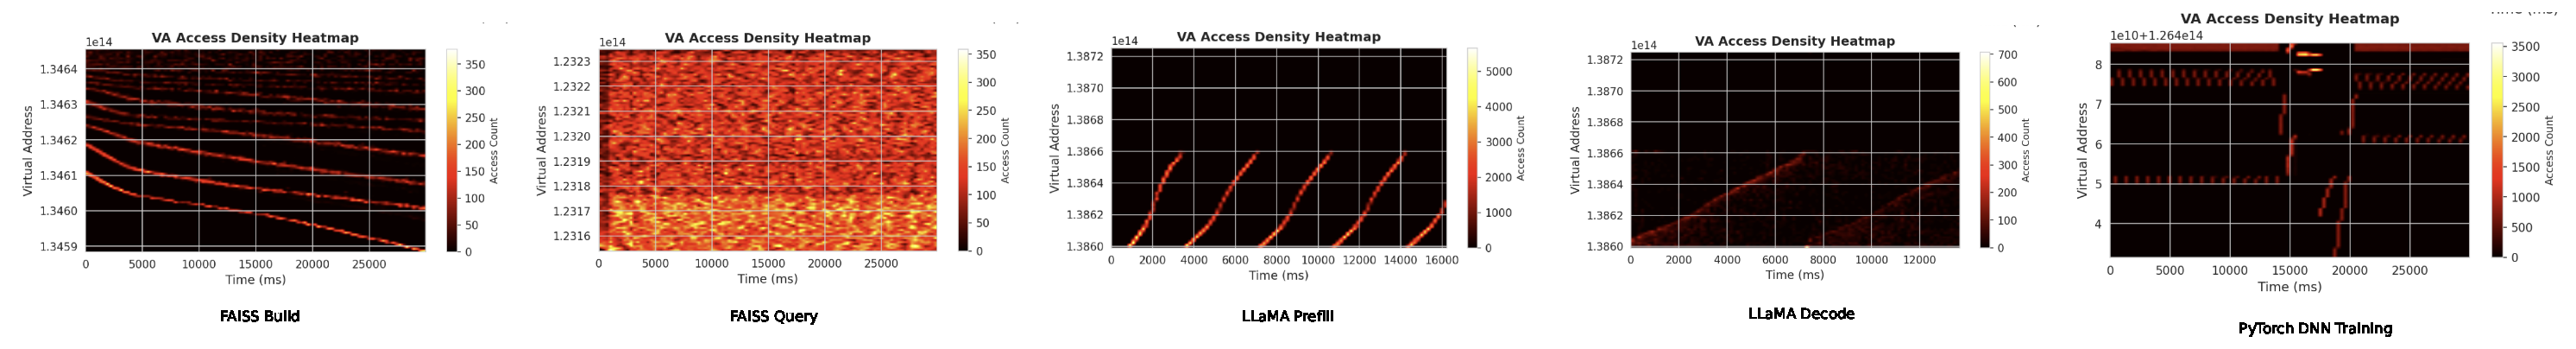
\includegraphics[width=\textwidth]{img/pattern/combined_patterns_1x5.pdf}
    \caption{Memory access(Page Fault) patterns vary significantly across GPU workloads. faiss Build exhibits sequential scans; faiss Query random accesses; llama.cpp MoE Prefill demonstrates periodic sequential patterns, and Decode exhibits more sparse random accesses; PyTorch DNN shows periodic block accesses. Such diversity necessitates adaptive memory management policies.}
    \label{fig:access_patterns}
\end{figure*}


\begin{figure}[t]
    \centering
    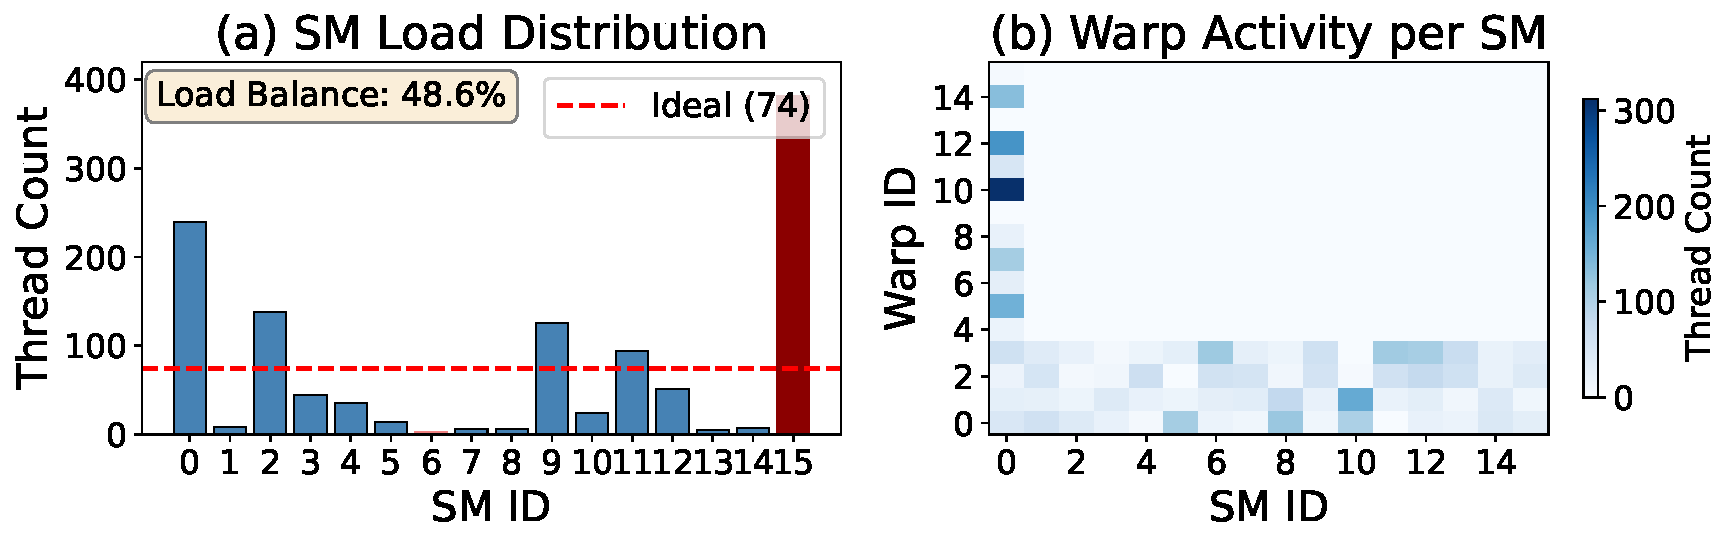
\includegraphics[width=\columnwidth]{img/pattern/vector_add/thread_scheduling_motivation.pdf}
    \caption{GPU thread scheduling imbalance observed via eBPF tracing. (a) SM load distribution shows 127$\times$ imbalance (SM~15: 382 threads vs SM~6: 3 threads). (b) Warp activity heatmap reveals SM~0 concentrates work in high-numbered warps while other SMs underutilize warp slots.}
    \label{fig:thread_scheduling}
\end{figure}

% \xiangyu{The following might need a little bit of rewriting. I do not know the relationship with the previous sentence. Does it mean the previous one needs schedulers not to treat per-GPU as black box? or treat different GPUs differently?}
% \yusheng{I think we can remove them.}
% \xiangyu{It is OK to roughly mention these scenarios (because people might have already known). However, instead of purely saying what they are doing, we should give one central sentence: they all generate heterogeneous workload.}

\subsection{GPU Systems Architecture}

\begin{figure}[t]
    \centering
    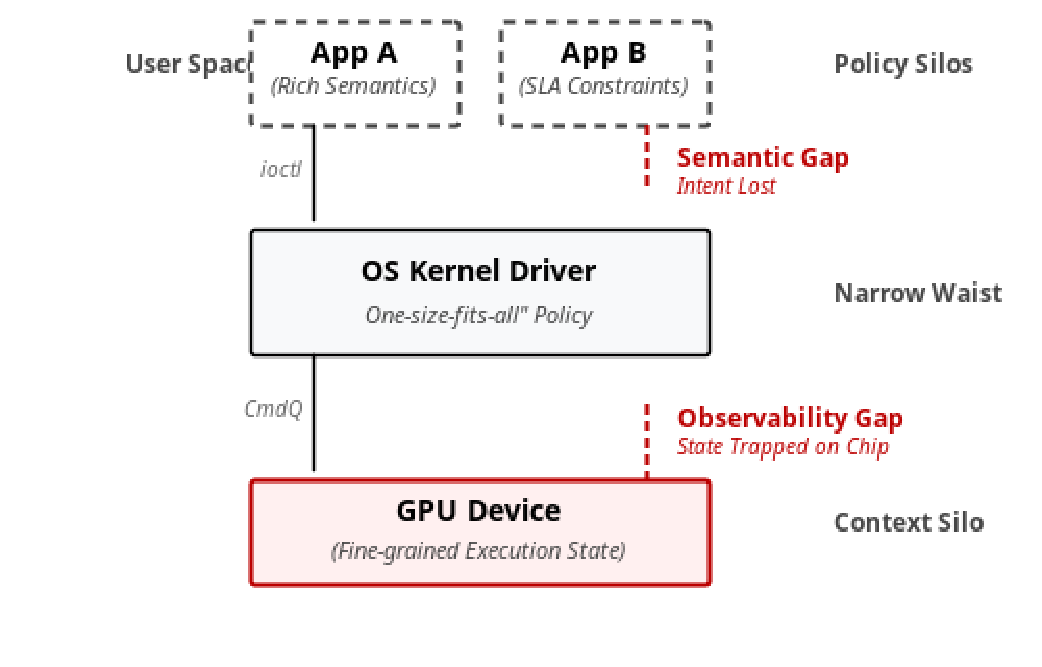
\includegraphics[width=\columnwidth]{img/motivation_silos.pdf}
    \caption{In modern GPU stacks, user-space applications have distinct requirements, but the OS driver is \emph{unprogrammable} and performs one-size-fits-all management. GPU device state remains \emph{invisible} to the host, preventing workload-aware policies.}
    \label{fig:motivation_silos}
\end{figure}

% need a better figure

% \xiangyu{High-level}
\paragraph{User-Space Logic (Applications \& Runtimes)}
% userspace include 2 parts: runtime and application. discuss them separately.
High-level frameworks (e.g., PyTorch) and runtime (e.g., CUDA libraries) operate in user space, managing operation graphs, tensor layouts, and command submissions. they possess rich semantic information (such as the structure of a neural network or the latency target of an inference query), and use memory map or  ioctl to talk with driver.
modern GPU systems like vLLM~\cite{kwon2023efficient} or custom runtimes implement complex memory and scheduler management logic entirely in user spaces. Fine-grained sharing frameworks such as Salus~\cite{salus} and UVM-focused runtimes like PILOT~\cite{pilot} likewise centralize time-sharing and memory placement decisions above the driver.

%Therefore, we believe we should leverage existing software and utilize eBPF to relatively easily add some flexibility, thus achieving the goal of programmability.
% 

\paragraph{The One-size-fits-all Kernel Driver}
As an os components, The GPU driver serves as the central authority for physical resource arbitration, holding exclusive control over the Memory Management Unit (MMU), hardware interrupts, and global context scheduling. Despite this privileged position, GPU drivers are typically monolithic, enforcing static, coarse-grained policies disconnected from workload-specific semantics. For memory management, the driver uses generic algorithms (e.g., LRU eviction and tree-based prefetching in Unified Virtual Memory) that overlook application-specific access patterns. For scheduling, it employs simple time-slicing (e.g., round-robin) to arbitrate between processes. This \emph{one-size-fits-all} management fundamentally limits performance optimization, acting as a primary bottleneck for tail latency and efficiency. 
    Prior OS-level work such as TimeGraph and Gdev moved GPU scheduling and memory control into Linux device drivers~\cite{kato2011timegraph,kato2012gdev}. More recent systems use kernel-space interception and preemptive scheduling (e.g., Zhang et al.~\cite{kernelintercept} and GPREEMPT~\cite{gpreempt}) to refactor driver-level control paths. However, these systems embed customized but fixed policies hard-coded in kernel modules, hindering rapid iteration, experimentation, or runtime adaptability. To overcome that, modern applications more similar to DPDK for network, choose to manage memory and schedule the request in userspace, rather than reply on driver algorithms.  LithOS~\cite{lithos} goes further by re-implementing portions of the GPU runtime stack with OS-like abstractions, but still operates entirely in user space, sacrificing direct access to privileged hardware events and still use one size fits all policy.
    \weichen{Complementing GPreempt, GCAPS~\cite{wang2024gcaps} demonstrates recent driver-level refactoring by implementing priority-based preemption for real-time guarantees. However, similar to prior approaches, GCAPS embeds a fixed scheduling policy within the driver, lacking a programmable interface for defining arbitrary resource management policies at runtime.}
% Updating drivers from scratch is extremely cumbersome, involving massive code updates, and could potentially introduce new bugs. Furthermore, much of the performance of driver software is application-scenario dependent, making it impossible to rewrite a driver for every new application scenario. 


\paragraph{Device-Side Execution}
Actual computation occurs on the GPU device, managed by a combination of user-written kernels (Device Code) and proprietary firmware, lacking runtime adaptability or transparency. Device kernels specify precise thread-level logic but compile into static binaries incapable of adapting dynamically to runtime conditions, such as cache contention or thread divergence. Meanwhile, the hardware scheduler manages the execution of thousands of threads (warps) but offers no programmable interface for prioritization. This creates \emph{execution opacity}: critical device states (e.g., warp divergence, cache thrashing) remain invisible to the host driver, severely restricting workload-adaptive optimization. In summary, modern GPU stacks suffer from tight coupling between resource management mechanisms (e.g., page migration, kernel execution lifecycle management, performance event collection) and embedded, hard-coded policy logic within kernel modules, closed-source vendor libraries or GPU device code. This tight coupling fundamentally constrains runtime flexibility, policy evolution, and the adaptability of GPU infrastructure in production environments.

\subsection{Limitations of Existing Extensibility Mechanisms}

% \xiangyu{I think we can simplify the description of various related works by only referencing them but not mentioning their details.
% Probably, it is better to highlight limitations.}

To mitigate this rigidity, developers currently resort to fragmented extensibility approaches:

\paragraph{Host User-Space Runtimes and Libraries}
More recent serving systems like Paella, Pie and KTransformers explicitly expose programmable interfaces: Paella provides software-defined GPU scheduling for model serving~\cite{paella}, Pie lets developers write ``inferlets'' that program the LLM generation loop and KV-cache management~\cite{pie}, and KTransformers offers a flexible CPU--GPU hybrid inference runtime with pluggable scheduling and expert-placement strategies~\cite{ktransformers}. XSched, although positioned as an XPU scheduling framework, also implements flexible, user-defined policies on top of its XQueue abstraction~\cite{xsched}. In this sense, many user-space systems are already programmable frameworks.

% \xiangyu{two limitations for these approaches:}
However, all of these approaches share three fundamental limitations for GPU resource management. First, their programmability is \emph{application-bound}: policies are written against a particular serving system or runtime, and cannot be reused across arbitrary applications or libraries without porting those applications onto the same stack. Second, user-space runtimes lack global coordination for resource sharing. Confined to process silos, they cannot safely share memory or bandwidth between tenants or mitigate interference from other tenants or frameworks. To avoid contention and faults, applications must conservatively pre-allocate resources (e.g., memory) at startup~\cite{lmcache}, preventing dynamic sharing and lowering utilization. Similarly, hardware partitioning techniques like MIG enforce fixed boundaries that cannot adapt to bursty traffic. Third, user-space systems lack fine-grained execution control. Operating above the driver, they lack a trusted, privileged interface to global low-level mechanisms such as page fault handling, MMU updates, and interrupt delivery. This confines policies to coarse-grained scheduling at kernel launch boundaries, preventing precise preemption for latency-sensitive tasks or fine-grained compute-transfer overlap. Moreover, they cannot operate on latency-critical paths such as page fault handlers, nor can they enforce policies sensitive to warp-level or barrier-level progress conditions (e.g., conditional preemption based on thread-block synchronization state) or GPU-side access patterns feeding into a driver-level region cache. Typically they require additional compiler integration to achieve this, making them non-transparent.

\paragraph{Binary Instrumentation and Profiling Tools on Device}
% \xiangyu{Three limitations for these tools:}
Tools like NVBit~\cite{nvbit}, Neutrino~\cite{neutrino} or sanitizer frameworks allow for the injection of logic directly into GPU binaries. NVBit provides dynamic SASS-level binary instrumentation for NVIDIA GPUs~\cite{nvbit}, while Neutrino attaches programmable probes at the assembly layer to profile kernels at instruction granularity with an eBPF-like user experience~\cite{neutrino}. While offering high visibility, these tools exhibit three key limitations. First, they lack strong safety guarantees: injected logic risks application crashes or hangs. Second, they are primarily designed for offline profiling rather than online policy enforcement, typically operating in a read-only manner and unable to actively regulate system behavior such as memory placement or thread scheduling. Third, they lack privileged driver integration; since many controls occur on the host side, they cannot coordinate policies beyond a single kernel. Instrumentation at the assembly level, as done by Neutrino, also inherently restricts policy expressiveness and portability. Recent user-space approaches like the eGPU workshop paper~\cite{egpu} demo extend eBPF to GPUs for observability, but remain limited to application-level instrumentation and incur prohibitive overheads (see \S\ref{sec:eval}).

\paragraph{Host-Based Kernel Programmability (CPU eBPF)}
The systems community has successfully used eBPF to customize OS policies on CPUs (e.g., \texttt{sched\_ext}, \texttt{cache\_ext}). However, directly extending this model to GPUs faces two fundamental barriers. First, host-based eBPF treats the GPU as an opaque peripheral; it can trace driver commands but remains blind to the device's internal execution state (e.g., warp divergence), making it impossible to react to on-chip bottlenecks. Second, unlike the Linux CPU scheduler which was refactored to support \texttt{sched\_ext}, monolithic GPU drivers lack safe, programmable extension points to dynamically change their runtime behavior. Retrofitting mechanism-policy separation into these drivers is non-trivial: resource management logic is tightly coupled with low-level hardware interactions (e.g., MMU invalidation sequences), and naively exposing these low-level mechanisms risks severe resource leaks, hardware hangs, or kernel panics, necessitating careful, safe interface design.

In summary, existing methods exhibit fundamental architectural asymmetry: host-side programmability lacks visibility into GPU-internal execution states and privileged interfaces, while device-side programmability is vendor-specific, opaque, and lacks safe host-side integration. This fundamental asymmetry severely limits the programmability, observability, and adaptability of GPU resource management across the system stack.
